% Created by tikzDevice version 0.12.3.1 on 2021-07-06 19:27:01
% !TEX encoding = UTF-8 Unicode
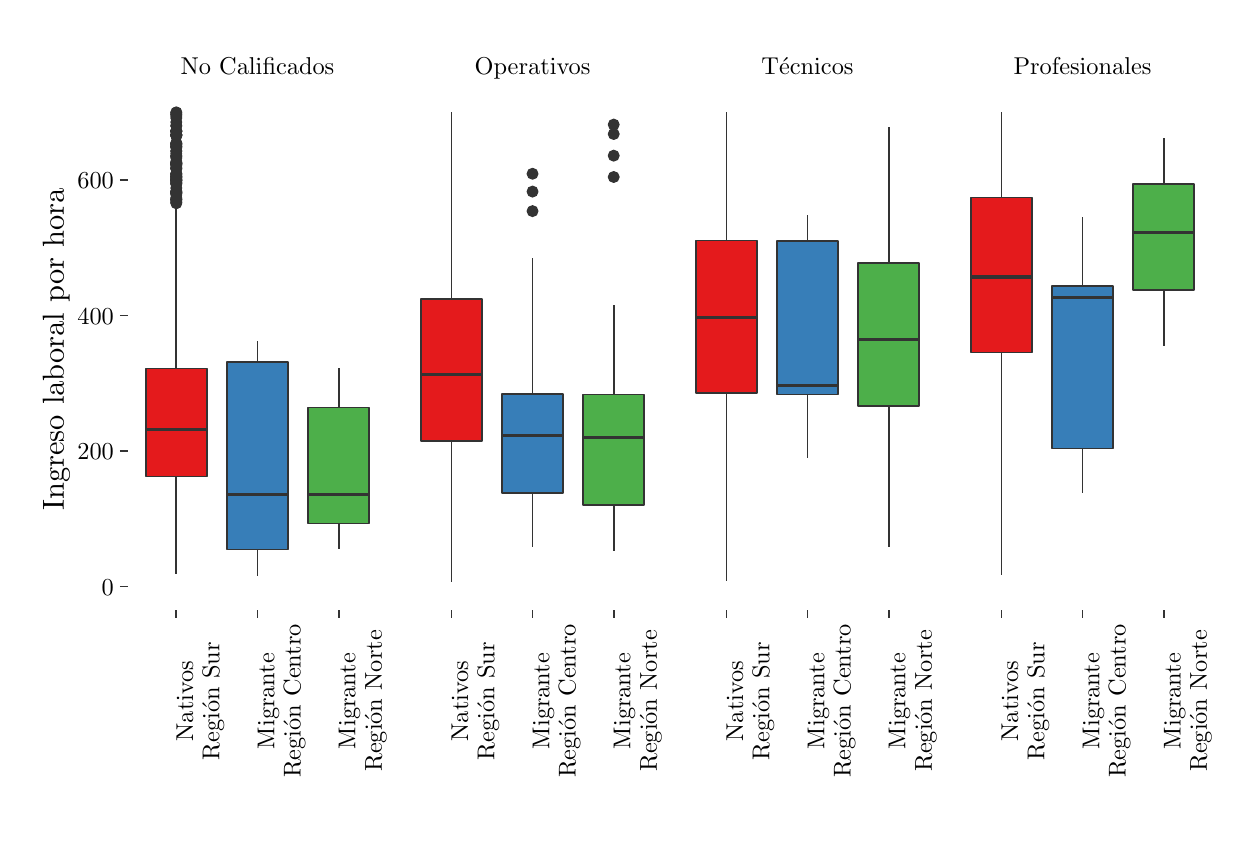
\begin{tikzpicture}[x=1pt,y=1pt]
\definecolor{fillColor}{RGB}{255,255,255}
\path[use as bounding box,fill=fillColor,fill opacity=0.00] (0,0) rectangle (433.62,289.08);
\begin{scope}
\path[clip] (  0.00,  0.00) rectangle (433.62,289.08);
\definecolor{drawColor}{RGB}{255,255,255}
\definecolor{fillColor}{RGB}{255,255,255}

\path[draw=drawColor,line width= 0.6pt,line join=round,line cap=round,fill=fillColor] (  0.00,  0.00) rectangle (433.62,289.08);
\end{scope}
\begin{scope}
\path[clip] ( 36.11, 78.54) rectangle (129.99,267.01);
\definecolor{drawColor}{RGB}{255,255,255}

\path[draw=drawColor,line width= 0.3pt,line join=round] ( 36.11,111.58) --
	(129.99,111.58);

\path[draw=drawColor,line width= 0.3pt,line join=round] ( 36.11,160.53) --
	(129.99,160.53);

\path[draw=drawColor,line width= 0.3pt,line join=round] ( 36.11,209.49) --
	(129.99,209.49);

\path[draw=drawColor,line width= 0.3pt,line join=round] ( 36.11,258.44) --
	(129.99,258.44);

\path[draw=drawColor,line width= 0.6pt,line join=round] ( 36.11, 87.10) --
	(129.99, 87.10);

\path[draw=drawColor,line width= 0.6pt,line join=round] ( 36.11,136.06) --
	(129.99,136.06);

\path[draw=drawColor,line width= 0.6pt,line join=round] ( 36.11,185.01) --
	(129.99,185.01);

\path[draw=drawColor,line width= 0.6pt,line join=round] ( 36.11,233.96) --
	(129.99,233.96);

\path[draw=drawColor,line width= 0.6pt,line join=round] ( 53.71, 78.54) --
	( 53.71,267.01);

\path[draw=drawColor,line width= 0.6pt,line join=round] ( 83.05, 78.54) --
	( 83.05,267.01);

\path[draw=drawColor,line width= 0.6pt,line join=round] (112.39, 78.54) --
	(112.39,267.01);
\definecolor{drawColor}{gray}{0.20}
\definecolor{fillColor}{gray}{0.20}

\path[draw=drawColor,line width= 0.4pt,line join=round,line cap=round,fill=fillColor] ( 53.71,236.11) circle (  1.96);

\path[draw=drawColor,line width= 0.4pt,line join=round,line cap=round,fill=fillColor] ( 53.71,242.67) circle (  1.96);

\path[draw=drawColor,line width= 0.4pt,line join=round,line cap=round,fill=fillColor] ( 53.71,236.11) circle (  1.96);

\path[draw=drawColor,line width= 0.4pt,line join=round,line cap=round,fill=fillColor] ( 53.71,243.57) circle (  1.96);

\path[draw=drawColor,line width= 0.4pt,line join=round,line cap=round,fill=fillColor] ( 53.71,239.49) circle (  1.96);

\path[draw=drawColor,line width= 0.4pt,line join=round,line cap=round,fill=fillColor] ( 53.71,256.43) circle (  1.96);

\path[draw=drawColor,line width= 0.4pt,line join=round,line cap=round,fill=fillColor] ( 53.71,251.59) circle (  1.96);

\path[draw=drawColor,line width= 0.4pt,line join=round,line cap=round,fill=fillColor] ( 53.71,229.33) circle (  1.96);

\path[draw=drawColor,line width= 0.4pt,line join=round,line cap=round,fill=fillColor] ( 53.71,226.97) circle (  1.96);

\path[draw=drawColor,line width= 0.4pt,line join=round,line cap=round,fill=fillColor] ( 53.71,226.97) circle (  1.96);

\path[draw=drawColor,line width= 0.4pt,line join=round,line cap=round,fill=fillColor] ( 53.71,226.97) circle (  1.96);

\path[draw=drawColor,line width= 0.4pt,line join=round,line cap=round,fill=fillColor] ( 53.71,236.29) circle (  1.96);

\path[draw=drawColor,line width= 0.4pt,line join=round,line cap=round,fill=fillColor] ( 53.71,240.05) circle (  1.96);

\path[draw=drawColor,line width= 0.4pt,line join=round,line cap=round,fill=fillColor] ( 53.71,227.62) circle (  1.96);

\path[draw=drawColor,line width= 0.4pt,line join=round,line cap=round,fill=fillColor] ( 53.71,226.06) circle (  1.96);

\path[draw=drawColor,line width= 0.4pt,line join=round,line cap=round,fill=fillColor] ( 53.71,226.06) circle (  1.96);

\path[draw=drawColor,line width= 0.4pt,line join=round,line cap=round,fill=fillColor] ( 53.71,246.11) circle (  1.96);

\path[draw=drawColor,line width= 0.4pt,line join=round,line cap=round,fill=fillColor] ( 53.71,246.11) circle (  1.96);

\path[draw=drawColor,line width= 0.4pt,line join=round,line cap=round,fill=fillColor] ( 53.71,246.11) circle (  1.96);

\path[draw=drawColor,line width= 0.4pt,line join=round,line cap=round,fill=fillColor] ( 53.71,232.48) circle (  1.96);

\path[draw=drawColor,line width= 0.4pt,line join=round,line cap=round,fill=fillColor] ( 53.71,235.51) circle (  1.96);

\path[draw=drawColor,line width= 0.4pt,line join=round,line cap=round,fill=fillColor] ( 53.71,238.16) circle (  1.96);

\path[draw=drawColor,line width= 0.4pt,line join=round,line cap=round,fill=fillColor] ( 53.71,238.16) circle (  1.96);

\path[draw=drawColor,line width= 0.4pt,line join=round,line cap=round,fill=fillColor] ( 53.71,233.39) circle (  1.96);

\path[draw=drawColor,line width= 0.4pt,line join=round,line cap=round,fill=fillColor] ( 53.71,242.83) circle (  1.96);

\path[draw=drawColor,line width= 0.4pt,line join=round,line cap=round,fill=fillColor] ( 53.71,239.65) circle (  1.96);

\path[draw=drawColor,line width= 0.4pt,line join=round,line cap=round,fill=fillColor] ( 53.71,234.57) circle (  1.96);

\path[draw=drawColor,line width= 0.4pt,line join=round,line cap=round,fill=fillColor] ( 53.71,229.48) circle (  1.96);

\path[draw=drawColor,line width= 0.4pt,line join=round,line cap=round,fill=fillColor] ( 53.71,235.41) circle (  1.96);

\path[draw=drawColor,line width= 0.4pt,line join=round,line cap=round,fill=fillColor] ( 53.71,247.13) circle (  1.96);

\path[draw=drawColor,line width= 0.4pt,line join=round,line cap=round,fill=fillColor] ( 53.71,251.70) circle (  1.96);

\path[draw=drawColor,line width= 0.4pt,line join=round,line cap=round,fill=fillColor] ( 53.71,251.70) circle (  1.96);

\path[draw=drawColor,line width= 0.4pt,line join=round,line cap=round,fill=fillColor] ( 53.71,251.70) circle (  1.96);

\path[draw=drawColor,line width= 0.4pt,line join=round,line cap=round,fill=fillColor] ( 53.71,247.13) circle (  1.96);

\path[draw=drawColor,line width= 0.4pt,line join=round,line cap=round,fill=fillColor] ( 53.71,240.73) circle (  1.96);

\path[draw=drawColor,line width= 0.4pt,line join=round,line cap=round,fill=fillColor] ( 53.71,247.13) circle (  1.96);

\path[draw=drawColor,line width= 0.4pt,line join=round,line cap=round,fill=fillColor] ( 53.71,231.12) circle (  1.96);

\path[draw=drawColor,line width= 0.4pt,line join=round,line cap=round,fill=fillColor] ( 53.71,232.85) circle (  1.96);

\path[draw=drawColor,line width= 0.4pt,line join=round,line cap=round,fill=fillColor] ( 53.71,250.34) circle (  1.96);

\path[draw=drawColor,line width= 0.4pt,line join=round,line cap=round,fill=fillColor] ( 53.71,250.34) circle (  1.96);

\path[draw=drawColor,line width= 0.4pt,line join=round,line cap=round,fill=fillColor] ( 53.71,244.51) circle (  1.96);

\path[draw=drawColor,line width= 0.4pt,line join=round,line cap=round,fill=fillColor] ( 53.71,238.68) circle (  1.96);

\path[draw=drawColor,line width= 0.4pt,line join=round,line cap=round,fill=fillColor] ( 53.71,232.85) circle (  1.96);

\path[draw=drawColor,line width= 0.4pt,line join=round,line cap=round,fill=fillColor] ( 53.71,257.14) circle (  1.96);

\path[draw=drawColor,line width= 0.4pt,line join=round,line cap=round,fill=fillColor] ( 53.71,229.32) circle (  1.96);

\path[draw=drawColor,line width= 0.4pt,line join=round,line cap=round,fill=fillColor] ( 53.71,238.21) circle (  1.96);

\path[draw=drawColor,line width= 0.4pt,line join=round,line cap=round,fill=fillColor] ( 53.71,257.76) circle (  1.96);

\path[draw=drawColor,line width= 0.4pt,line join=round,line cap=round,fill=fillColor] ( 53.71,229.32) circle (  1.96);

\path[draw=drawColor,line width= 0.4pt,line join=round,line cap=round,fill=fillColor] ( 53.71,225.62) circle (  1.96);

\path[draw=drawColor,line width= 0.4pt,line join=round,line cap=round,fill=fillColor] ( 53.71,236.43) circle (  1.96);

\path[draw=drawColor,line width= 0.4pt,line join=round,line cap=round,fill=fillColor] ( 53.71,251.67) circle (  1.96);

\path[draw=drawColor,line width= 0.4pt,line join=round,line cap=round,fill=fillColor] ( 53.71,239.48) circle (  1.96);

\path[draw=drawColor,line width= 0.4pt,line join=round,line cap=round,fill=fillColor] ( 53.71,251.67) circle (  1.96);

\path[draw=drawColor,line width= 0.4pt,line join=round,line cap=round,fill=fillColor] ( 53.71,257.76) circle (  1.96);

\path[draw=drawColor,line width= 0.4pt,line join=round,line cap=round,fill=fillColor] ( 53.71,233.01) circle (  1.96);

\path[draw=drawColor,line width= 0.4pt,line join=round,line cap=round,fill=fillColor] ( 53.71,246.97) circle (  1.96);

\path[draw=drawColor,line width= 0.4pt,line join=round,line cap=round,fill=fillColor] ( 53.71,235.12) circle (  1.96);

\path[draw=drawColor,line width= 0.4pt,line join=round,line cap=round,fill=fillColor] ( 53.71,242.53) circle (  1.96);

\path[draw=drawColor,line width= 0.4pt,line join=round,line cap=round,fill=fillColor] ( 53.71,245.70) circle (  1.96);

\path[draw=drawColor,line width= 0.4pt,line join=round,line cap=round,fill=fillColor] ( 53.71,235.12) circle (  1.96);

\path[draw=drawColor,line width= 0.4pt,line join=round,line cap=round,fill=fillColor] ( 53.71,249.93) circle (  1.96);

\path[draw=drawColor,line width= 0.4pt,line join=round,line cap=round,fill=fillColor] ( 53.71,253.63) circle (  1.96);

\path[draw=drawColor,line width= 0.4pt,line join=round,line cap=round,fill=fillColor] ( 53.71,253.63) circle (  1.96);

\path[draw=drawColor,line width= 0.4pt,line join=round,line cap=round,fill=fillColor] ( 53.71,235.12) circle (  1.96);

\path[draw=drawColor,line width= 0.4pt,line join=round,line cap=round,fill=fillColor] ( 53.71,247.46) circle (  1.96);

\path[draw=drawColor,line width= 0.4pt,line join=round,line cap=round,fill=fillColor] ( 53.71,244.45) circle (  1.96);

\path[draw=drawColor,line width= 0.4pt,line join=round,line cap=round,fill=fillColor] ( 53.71,246.42) circle (  1.96);

\path[draw=drawColor,line width= 0.4pt,line join=round,line cap=round,fill=fillColor] ( 53.71,234.62) circle (  1.96);

\path[draw=drawColor,line width= 0.4pt,line join=round,line cap=round,fill=fillColor] ( 53.71,241.99) circle (  1.96);

\path[draw=drawColor,line width= 0.4pt,line join=round,line cap=round,fill=fillColor] ( 53.71,228.71) circle (  1.96);

\path[draw=drawColor,line width= 0.4pt,line join=round,line cap=round,fill=fillColor] ( 53.71,254.94) circle (  1.96);

\path[draw=drawColor,line width= 0.4pt,line join=round,line cap=round,fill=fillColor] ( 53.71,233.96) circle (  1.96);

\path[draw=drawColor,line width= 0.4pt,line join=round,line cap=round,fill=fillColor] ( 53.71,229.89) circle (  1.96);

\path[draw=drawColor,line width= 0.4pt,line join=round,line cap=round,fill=fillColor] ( 53.71,240.08) circle (  1.96);

\path[draw=drawColor,line width= 0.4pt,line join=round,line cap=round,fill=fillColor] ( 53.71,240.08) circle (  1.96);

\path[draw=drawColor,line width= 0.4pt,line join=round,line cap=round,fill=fillColor] ( 53.71,250.28) circle (  1.96);

\path[draw=drawColor,line width= 0.4pt,line join=round,line cap=round,fill=fillColor] ( 53.71,250.28) circle (  1.96);

\path[draw=drawColor,line width= 0.4pt,line join=round,line cap=round,fill=fillColor] ( 53.71,233.96) circle (  1.96);

\path[draw=drawColor,line width= 0.4pt,line join=round,line cap=round,fill=fillColor] ( 53.71,240.08) circle (  1.96);

\path[draw=drawColor,line width= 0.4pt,line join=round,line cap=round,fill=fillColor] ( 53.71,229.89) circle (  1.96);

\path[draw=drawColor,line width= 0.4pt,line join=round,line cap=round,fill=fillColor] ( 53.71,229.89) circle (  1.96);

\path[draw=drawColor,line width= 0.4pt,line join=round,line cap=round,fill=fillColor] ( 53.71,240.08) circle (  1.96);

\path[draw=drawColor,line width= 0.4pt,line join=round,line cap=round,fill=fillColor] ( 53.71,233.96) circle (  1.96);

\path[draw=drawColor,line width= 0.4pt,line join=round,line cap=round,fill=fillColor] ( 53.71,226.97) circle (  1.96);

\path[draw=drawColor,line width= 0.4pt,line join=round,line cap=round,fill=fillColor] ( 53.71,250.28) circle (  1.96);

\path[draw=drawColor,line width= 0.4pt,line join=round,line cap=round,fill=fillColor] ( 53.71,250.28) circle (  1.96);

\path[draw=drawColor,line width= 0.4pt,line join=round,line cap=round,fill=fillColor] ( 53.71,240.08) circle (  1.96);

\path[draw=drawColor,line width= 0.4pt,line join=round,line cap=round,fill=fillColor] ( 53.71,233.96) circle (  1.96);

\path[draw=drawColor,line width= 0.4pt,line join=round,line cap=round,fill=fillColor] ( 53.71,258.44) circle (  1.96);

\path[draw=drawColor,line width= 0.4pt,line join=round,line cap=round,fill=fillColor] ( 53.71,258.44) circle (  1.96);

\path[draw=drawColor,line width= 0.4pt,line join=round,line cap=round,fill=fillColor] ( 53.71,233.96) circle (  1.96);

\path[draw=drawColor,line width= 0.4pt,line join=round,line cap=round,fill=fillColor] ( 53.71,233.96) circle (  1.96);

\path[draw=drawColor,line width= 0.6pt,line join=round] ( 53.71,165.97) -- ( 53.71,224.29);

\path[draw=drawColor,line width= 0.6pt,line join=round] ( 53.71,126.88) -- ( 53.71, 91.69);
\definecolor{fillColor}{RGB}{228,26,28}

\path[draw=drawColor,line width= 0.6pt,line join=round,line cap=round,fill=fillColor] ( 42.71,165.97) --
	( 42.71,126.88) --
	( 64.71,126.88) --
	( 64.71,165.97) --
	( 42.71,165.97) --
	cycle;

\path[draw=drawColor,line width= 1.1pt,line join=round] ( 42.71,143.99) -- ( 64.71,143.99);

\path[draw=drawColor,line width= 0.6pt,line join=round] ( 83.05,168.38) -- ( 83.05,175.92);

\path[draw=drawColor,line width= 0.6pt,line join=round] ( 83.05,100.49) -- ( 83.05, 91.08);
\definecolor{fillColor}{RGB}{55,126,184}

\path[draw=drawColor,line width= 0.6pt,line join=round,line cap=round,fill=fillColor] ( 72.05,168.38) --
	( 72.05,100.49) --
	( 94.05,100.49) --
	( 94.05,168.38) --
	( 72.05,168.38) --
	cycle;

\path[draw=drawColor,line width= 1.1pt,line join=round] ( 72.05,120.23) -- ( 94.05,120.23);

\path[draw=drawColor,line width= 0.6pt,line join=round] (112.39,151.87) -- (112.39,166.20);

\path[draw=drawColor,line width= 0.6pt,line join=round] (112.39,109.96) -- (112.39,100.82);
\definecolor{fillColor}{RGB}{77,175,74}

\path[draw=drawColor,line width= 0.6pt,line join=round,line cap=round,fill=fillColor] (101.39,151.87) --
	(101.39,109.96) --
	(123.39,109.96) --
	(123.39,151.87) --
	(101.39,151.87) --
	cycle;

\path[draw=drawColor,line width= 1.1pt,line join=round] (101.39,120.47) -- (123.39,120.47);
\end{scope}
\begin{scope}
\path[clip] (135.49, 78.54) rectangle (229.37,267.01);
\definecolor{drawColor}{RGB}{255,255,255}

\path[draw=drawColor,line width= 0.3pt,line join=round] (135.49,111.58) --
	(229.37,111.58);

\path[draw=drawColor,line width= 0.3pt,line join=round] (135.49,160.53) --
	(229.37,160.53);

\path[draw=drawColor,line width= 0.3pt,line join=round] (135.49,209.49) --
	(229.37,209.49);

\path[draw=drawColor,line width= 0.3pt,line join=round] (135.49,258.44) --
	(229.37,258.44);

\path[draw=drawColor,line width= 0.6pt,line join=round] (135.49, 87.10) --
	(229.37, 87.10);

\path[draw=drawColor,line width= 0.6pt,line join=round] (135.49,136.06) --
	(229.37,136.06);

\path[draw=drawColor,line width= 0.6pt,line join=round] (135.49,185.01) --
	(229.37,185.01);

\path[draw=drawColor,line width= 0.6pt,line join=round] (135.49,233.96) --
	(229.37,233.96);

\path[draw=drawColor,line width= 0.6pt,line join=round] (153.09, 78.54) --
	(153.09,267.01);

\path[draw=drawColor,line width= 0.6pt,line join=round] (182.43, 78.54) --
	(182.43,267.01);

\path[draw=drawColor,line width= 0.6pt,line join=round] (211.76, 78.54) --
	(211.76,267.01);
\definecolor{drawColor}{gray}{0.20}

\path[draw=drawColor,line width= 0.6pt,line join=round] (153.09,190.92) -- (153.09,258.44);

\path[draw=drawColor,line width= 0.6pt,line join=round] (153.09,139.81) -- (153.09, 88.88);
\definecolor{fillColor}{RGB}{228,26,28}

\path[draw=drawColor,line width= 0.6pt,line join=round,line cap=round,fill=fillColor] (142.09,190.92) --
	(142.09,139.81) --
	(164.09,139.81) --
	(164.09,190.92) --
	(142.09,190.92) --
	cycle;

\path[draw=drawColor,line width= 1.1pt,line join=round] (142.09,163.62) -- (164.09,163.62);
\definecolor{fillColor}{gray}{0.20}

\path[draw=drawColor,line width= 0.4pt,line join=round,line cap=round,fill=fillColor] (182.43,236.29) circle (  1.96);

\path[draw=drawColor,line width= 0.4pt,line join=round,line cap=round,fill=fillColor] (182.43,229.85) circle (  1.96);

\path[draw=drawColor,line width= 0.4pt,line join=round,line cap=round,fill=fillColor] (182.43,222.79) circle (  1.96);

\path[draw=drawColor,line width= 0.6pt,line join=round] (182.43,156.63) -- (182.43,205.75);

\path[draw=drawColor,line width= 0.6pt,line join=round] (182.43,121.01) -- (182.43,101.41);
\definecolor{fillColor}{RGB}{55,126,184}

\path[draw=drawColor,line width= 0.6pt,line join=round,line cap=round,fill=fillColor] (171.43,156.63) --
	(171.43,121.01) --
	(193.43,121.01) --
	(193.43,156.63) --
	(171.43,156.63) --
	cycle;

\path[draw=drawColor,line width= 1.1pt,line join=round] (171.43,141.67) -- (193.43,141.67);
\definecolor{fillColor}{gray}{0.20}

\path[draw=drawColor,line width= 0.4pt,line join=round,line cap=round,fill=fillColor] (211.76,254.06) circle (  1.96);

\path[draw=drawColor,line width= 0.4pt,line join=round,line cap=round,fill=fillColor] (211.76,242.83) circle (  1.96);

\path[draw=drawColor,line width= 0.4pt,line join=round,line cap=round,fill=fillColor] (211.76,250.65) circle (  1.96);

\path[draw=drawColor,line width= 0.4pt,line join=round,line cap=round,fill=fillColor] (211.76,235.12) circle (  1.96);

\path[draw=drawColor,line width= 0.6pt,line join=round] (211.76,156.58) -- (211.76,188.70);

\path[draw=drawColor,line width= 0.6pt,line join=round] (211.76,116.60) -- (211.76, 99.80);
\definecolor{fillColor}{RGB}{77,175,74}

\path[draw=drawColor,line width= 0.6pt,line join=round,line cap=round,fill=fillColor] (200.76,156.58) --
	(200.76,116.60) --
	(222.76,116.60) --
	(222.76,156.58) --
	(200.76,156.58) --
	cycle;

\path[draw=drawColor,line width= 1.1pt,line join=round] (200.76,140.95) -- (222.76,140.95);
\end{scope}
\begin{scope}
\path[clip] (234.87, 78.54) rectangle (328.74,267.01);
\definecolor{drawColor}{RGB}{255,255,255}

\path[draw=drawColor,line width= 0.3pt,line join=round] (234.87,111.58) --
	(328.74,111.58);

\path[draw=drawColor,line width= 0.3pt,line join=round] (234.87,160.53) --
	(328.74,160.53);

\path[draw=drawColor,line width= 0.3pt,line join=round] (234.87,209.49) --
	(328.74,209.49);

\path[draw=drawColor,line width= 0.3pt,line join=round] (234.87,258.44) --
	(328.74,258.44);

\path[draw=drawColor,line width= 0.6pt,line join=round] (234.87, 87.10) --
	(328.74, 87.10);

\path[draw=drawColor,line width= 0.6pt,line join=round] (234.87,136.06) --
	(328.74,136.06);

\path[draw=drawColor,line width= 0.6pt,line join=round] (234.87,185.01) --
	(328.74,185.01);

\path[draw=drawColor,line width= 0.6pt,line join=round] (234.87,233.96) --
	(328.74,233.96);

\path[draw=drawColor,line width= 0.6pt,line join=round] (252.47, 78.54) --
	(252.47,267.01);

\path[draw=drawColor,line width= 0.6pt,line join=round] (281.80, 78.54) --
	(281.80,267.01);

\path[draw=drawColor,line width= 0.6pt,line join=round] (311.14, 78.54) --
	(311.14,267.01);
\definecolor{drawColor}{gray}{0.20}

\path[draw=drawColor,line width= 0.6pt,line join=round] (252.47,212.19) -- (252.47,258.44);

\path[draw=drawColor,line width= 0.6pt,line join=round] (252.47,157.03) -- (252.47, 88.98);
\definecolor{fillColor}{RGB}{228,26,28}

\path[draw=drawColor,line width= 0.6pt,line join=round,line cap=round,fill=fillColor] (241.47,212.19) --
	(241.47,157.03) --
	(263.47,157.03) --
	(263.47,212.19) --
	(241.47,212.19) --
	cycle;

\path[draw=drawColor,line width= 1.1pt,line join=round] (241.47,184.37) -- (263.47,184.37);

\path[draw=drawColor,line width= 0.6pt,line join=round] (281.80,212.00) -- (281.80,221.52);

\path[draw=drawColor,line width= 0.6pt,line join=round] (281.80,156.58) -- (281.80,133.42);
\definecolor{fillColor}{RGB}{55,126,184}

\path[draw=drawColor,line width= 0.6pt,line join=round,line cap=round,fill=fillColor] (270.80,212.00) --
	(270.80,156.58) --
	(292.81,156.58) --
	(292.81,212.00) --
	(270.80,212.00) --
	cycle;

\path[draw=drawColor,line width= 1.1pt,line join=round] (270.80,159.83) -- (292.81,159.83);

\path[draw=drawColor,line width= 0.6pt,line join=round] (311.14,204.05) -- (311.14,253.02);

\path[draw=drawColor,line width= 0.6pt,line join=round] (311.14,152.36) -- (311.14,101.32);
\definecolor{fillColor}{RGB}{77,175,74}

\path[draw=drawColor,line width= 0.6pt,line join=round,line cap=round,fill=fillColor] (300.14,204.05) --
	(300.14,152.36) --
	(322.14,152.36) --
	(322.14,204.05) --
	(300.14,204.05) --
	cycle;

\path[draw=drawColor,line width= 1.1pt,line join=round] (300.14,176.44) -- (322.14,176.44);
\end{scope}
\begin{scope}
\path[clip] (334.24, 78.54) rectangle (428.12,267.01);
\definecolor{drawColor}{RGB}{255,255,255}

\path[draw=drawColor,line width= 0.3pt,line join=round] (334.24,111.58) --
	(428.12,111.58);

\path[draw=drawColor,line width= 0.3pt,line join=round] (334.24,160.53) --
	(428.12,160.53);

\path[draw=drawColor,line width= 0.3pt,line join=round] (334.24,209.49) --
	(428.12,209.49);

\path[draw=drawColor,line width= 0.3pt,line join=round] (334.24,258.44) --
	(428.12,258.44);

\path[draw=drawColor,line width= 0.6pt,line join=round] (334.24, 87.10) --
	(428.12, 87.10);

\path[draw=drawColor,line width= 0.6pt,line join=round] (334.24,136.06) --
	(428.12,136.06);

\path[draw=drawColor,line width= 0.6pt,line join=round] (334.24,185.01) --
	(428.12,185.01);

\path[draw=drawColor,line width= 0.6pt,line join=round] (334.24,233.96) --
	(428.12,233.96);

\path[draw=drawColor,line width= 0.6pt,line join=round] (351.84, 78.54) --
	(351.84,267.01);

\path[draw=drawColor,line width= 0.6pt,line join=round] (381.18, 78.54) --
	(381.18,267.01);

\path[draw=drawColor,line width= 0.6pt,line join=round] (410.52, 78.54) --
	(410.52,267.01);
\definecolor{drawColor}{gray}{0.20}

\path[draw=drawColor,line width= 0.6pt,line join=round] (351.84,227.73) -- (351.84,258.44);

\path[draw=drawColor,line width= 0.6pt,line join=round] (351.84,171.76) -- (351.84, 91.37);
\definecolor{fillColor}{RGB}{228,26,28}

\path[draw=drawColor,line width= 0.6pt,line join=round,line cap=round,fill=fillColor] (340.84,227.73) --
	(340.84,171.76) --
	(362.85,171.76) --
	(362.85,227.73) --
	(340.84,227.73) --
	cycle;

\path[draw=drawColor,line width= 1.1pt,line join=round] (340.84,198.99) -- (362.85,198.99);

\path[draw=drawColor,line width= 0.6pt,line join=round] (381.18,195.66) -- (381.18,220.58);

\path[draw=drawColor,line width= 0.6pt,line join=round] (381.18,137.06) -- (381.18,121.07);
\definecolor{fillColor}{RGB}{55,126,184}

\path[draw=drawColor,line width= 0.6pt,line join=round,line cap=round,fill=fillColor] (370.18,195.66) --
	(370.18,137.06) --
	(392.18,137.06) --
	(392.18,195.66) --
	(370.18,195.66) --
	cycle;

\path[draw=drawColor,line width= 1.1pt,line join=round] (370.18,191.44) -- (392.18,191.44);

\path[draw=drawColor,line width= 0.6pt,line join=round] (410.52,232.67) -- (410.52,249.22);

\path[draw=drawColor,line width= 0.6pt,line join=round] (410.52,194.28) -- (410.52,173.95);
\definecolor{fillColor}{RGB}{77,175,74}

\path[draw=drawColor,line width= 0.6pt,line join=round,line cap=round,fill=fillColor] (399.52,232.67) --
	(399.52,194.28) --
	(421.52,194.28) --
	(421.52,232.67) --
	(399.52,232.67) --
	cycle;

\path[draw=drawColor,line width= 1.1pt,line join=round] (399.52,215.12) -- (421.52,215.12);
\end{scope}
\begin{scope}
\path[clip] ( 36.11,267.01) rectangle (129.99,283.58);
\definecolor{drawColor}{RGB}{0,0,0}

\node[text=drawColor,anchor=base,inner sep=0pt, outer sep=0pt, scale=  0.88] at ( 83.05,272.26) {No Calificados};
\end{scope}
\begin{scope}
\path[clip] (135.49,267.01) rectangle (229.37,283.58);
\definecolor{drawColor}{RGB}{0,0,0}

\node[text=drawColor,anchor=base,inner sep=0pt, outer sep=0pt, scale=  0.88] at (182.43,272.26) {Operativos};
\end{scope}
\begin{scope}
\path[clip] (234.87,267.01) rectangle (328.74,283.58);
\definecolor{drawColor}{RGB}{0,0,0}

\node[text=drawColor,anchor=base,inner sep=0pt, outer sep=0pt, scale=  0.88] at (281.80,272.26) {Técnicos};
\end{scope}
\begin{scope}
\path[clip] (334.24,267.01) rectangle (428.12,283.58);
\definecolor{drawColor}{RGB}{0,0,0}

\node[text=drawColor,anchor=base,inner sep=0pt, outer sep=0pt, scale=  0.88] at (381.18,272.26) {Profesionales};
\end{scope}
\begin{scope}
\path[clip] (  0.00,  0.00) rectangle (433.62,289.08);
\definecolor{drawColor}{gray}{0.20}

\path[draw=drawColor,line width= 0.6pt,line join=round] ( 53.71, 75.79) --
	( 53.71, 78.54);

\path[draw=drawColor,line width= 0.6pt,line join=round] ( 83.05, 75.79) --
	( 83.05, 78.54);

\path[draw=drawColor,line width= 0.6pt,line join=round] (112.39, 75.79) --
	(112.39, 78.54);
\end{scope}
\begin{scope}
\path[clip] (  0.00,  0.00) rectangle (433.62,289.08);
\definecolor{drawColor}{RGB}{0,0,0}

\node[text=drawColor,rotate= 90.00,anchor=base,inner sep=0pt, outer sep=0pt, scale=  0.88] at ( 59.77, 45.78) {Nativos};

\node[text=drawColor,rotate= 90.00,anchor=base,inner sep=0pt, outer sep=0pt, scale=  0.88] at ( 69.28, 45.78) {Región Sur};

\node[text=drawColor,rotate= 90.00,anchor=base,inner sep=0pt, outer sep=0pt, scale=  0.88] at ( 89.11, 45.78) {Migrante};

\node[text=drawColor,rotate= 90.00,anchor=base,inner sep=0pt, outer sep=0pt, scale=  0.88] at ( 98.61, 45.78) {Región Centro};

\node[text=drawColor,rotate= 90.00,anchor=base,inner sep=0pt, outer sep=0pt, scale=  0.88] at (118.45, 45.78) {Migrante};

\node[text=drawColor,rotate= 90.00,anchor=base,inner sep=0pt, outer sep=0pt, scale=  0.88] at (127.95, 45.78) {Región Norte};
\end{scope}
\begin{scope}
\path[clip] (  0.00,  0.00) rectangle (433.62,289.08);
\definecolor{drawColor}{gray}{0.20}

\path[draw=drawColor,line width= 0.6pt,line join=round] (153.09, 75.79) --
	(153.09, 78.54);

\path[draw=drawColor,line width= 0.6pt,line join=round] (182.43, 75.79) --
	(182.43, 78.54);

\path[draw=drawColor,line width= 0.6pt,line join=round] (211.76, 75.79) --
	(211.76, 78.54);
\end{scope}
\begin{scope}
\path[clip] (  0.00,  0.00) rectangle (433.62,289.08);
\definecolor{drawColor}{RGB}{0,0,0}

\node[text=drawColor,rotate= 90.00,anchor=base,inner sep=0pt, outer sep=0pt, scale=  0.88] at (159.15, 45.78) {Nativos};

\node[text=drawColor,rotate= 90.00,anchor=base,inner sep=0pt, outer sep=0pt, scale=  0.88] at (168.66, 45.78) {Región Sur};

\node[text=drawColor,rotate= 90.00,anchor=base,inner sep=0pt, outer sep=0pt, scale=  0.88] at (188.49, 45.78) {Migrante};

\node[text=drawColor,rotate= 90.00,anchor=base,inner sep=0pt, outer sep=0pt, scale=  0.88] at (197.99, 45.78) {Región Centro};

\node[text=drawColor,rotate= 90.00,anchor=base,inner sep=0pt, outer sep=0pt, scale=  0.88] at (217.82, 45.78) {Migrante};

\node[text=drawColor,rotate= 90.00,anchor=base,inner sep=0pt, outer sep=0pt, scale=  0.88] at (227.33, 45.78) {Región Norte};
\end{scope}
\begin{scope}
\path[clip] (  0.00,  0.00) rectangle (433.62,289.08);
\definecolor{drawColor}{gray}{0.20}

\path[draw=drawColor,line width= 0.6pt,line join=round] (252.47, 75.79) --
	(252.47, 78.54);

\path[draw=drawColor,line width= 0.6pt,line join=round] (281.80, 75.79) --
	(281.80, 78.54);

\path[draw=drawColor,line width= 0.6pt,line join=round] (311.14, 75.79) --
	(311.14, 78.54);
\end{scope}
\begin{scope}
\path[clip] (  0.00,  0.00) rectangle (433.62,289.08);
\definecolor{drawColor}{RGB}{0,0,0}

\node[text=drawColor,rotate= 90.00,anchor=base,inner sep=0pt, outer sep=0pt, scale=  0.88] at (258.53, 45.78) {Nativos};

\node[text=drawColor,rotate= 90.00,anchor=base,inner sep=0pt, outer sep=0pt, scale=  0.88] at (268.03, 45.78) {Región Sur};

\node[text=drawColor,rotate= 90.00,anchor=base,inner sep=0pt, outer sep=0pt, scale=  0.88] at (287.86, 45.78) {Migrante};

\node[text=drawColor,rotate= 90.00,anchor=base,inner sep=0pt, outer sep=0pt, scale=  0.88] at (297.37, 45.78) {Región Centro};

\node[text=drawColor,rotate= 90.00,anchor=base,inner sep=0pt, outer sep=0pt, scale=  0.88] at (317.20, 45.78) {Migrante};

\node[text=drawColor,rotate= 90.00,anchor=base,inner sep=0pt, outer sep=0pt, scale=  0.88] at (326.71, 45.78) {Región Norte};
\end{scope}
\begin{scope}
\path[clip] (  0.00,  0.00) rectangle (433.62,289.08);
\definecolor{drawColor}{gray}{0.20}

\path[draw=drawColor,line width= 0.6pt,line join=round] (351.84, 75.79) --
	(351.84, 78.54);

\path[draw=drawColor,line width= 0.6pt,line join=round] (381.18, 75.79) --
	(381.18, 78.54);

\path[draw=drawColor,line width= 0.6pt,line join=round] (410.52, 75.79) --
	(410.52, 78.54);
\end{scope}
\begin{scope}
\path[clip] (  0.00,  0.00) rectangle (433.62,289.08);
\definecolor{drawColor}{RGB}{0,0,0}

\node[text=drawColor,rotate= 90.00,anchor=base,inner sep=0pt, outer sep=0pt, scale=  0.88] at (357.91, 45.78) {Nativos};

\node[text=drawColor,rotate= 90.00,anchor=base,inner sep=0pt, outer sep=0pt, scale=  0.88] at (367.41, 45.78) {Región Sur};

\node[text=drawColor,rotate= 90.00,anchor=base,inner sep=0pt, outer sep=0pt, scale=  0.88] at (387.24, 45.78) {Migrante};

\node[text=drawColor,rotate= 90.00,anchor=base,inner sep=0pt, outer sep=0pt, scale=  0.88] at (396.75, 45.78) {Región Centro};

\node[text=drawColor,rotate= 90.00,anchor=base,inner sep=0pt, outer sep=0pt, scale=  0.88] at (416.58, 45.78) {Migrante};

\node[text=drawColor,rotate= 90.00,anchor=base,inner sep=0pt, outer sep=0pt, scale=  0.88] at (426.08, 45.78) {Región Norte};
\end{scope}
\begin{scope}
\path[clip] (  0.00,  0.00) rectangle (433.62,289.08);
\definecolor{drawColor}{RGB}{0,0,0}

\node[text=drawColor,anchor=base east,inner sep=0pt, outer sep=0pt, scale=  0.88] at ( 31.16, 84.07) {0};

\node[text=drawColor,anchor=base east,inner sep=0pt, outer sep=0pt, scale=  0.88] at ( 31.16,133.03) {200};

\node[text=drawColor,anchor=base east,inner sep=0pt, outer sep=0pt, scale=  0.88] at ( 31.16,181.98) {400};

\node[text=drawColor,anchor=base east,inner sep=0pt, outer sep=0pt, scale=  0.88] at ( 31.16,230.93) {600};
\end{scope}
\begin{scope}
\path[clip] (  0.00,  0.00) rectangle (433.62,289.08);
\definecolor{drawColor}{gray}{0.20}

\path[draw=drawColor,line width= 0.6pt,line join=round] ( 33.36, 87.10) --
	( 36.11, 87.10);

\path[draw=drawColor,line width= 0.6pt,line join=round] ( 33.36,136.06) --
	( 36.11,136.06);

\path[draw=drawColor,line width= 0.6pt,line join=round] ( 33.36,185.01) --
	( 36.11,185.01);

\path[draw=drawColor,line width= 0.6pt,line join=round] ( 33.36,233.96) --
	( 36.11,233.96);
\end{scope}
\begin{scope}
\path[clip] (  0.00,  0.00) rectangle (433.62,289.08);
\definecolor{drawColor}{RGB}{0,0,0}

\node[text=drawColor,rotate= 90.00,anchor=base,inner sep=0pt, outer sep=0pt, scale=  1.10] at ( 13.08,172.77) {Ingreso laboral por hora};
\end{scope}
\end{tikzpicture}
